




\section*{Simulation}
\subsection*{Why Simulate}
To test the system it is much better to simulate the given system instead of doing testing on the real system. That is because then one can do testing without destroying expensive equipment and if multiple people are working on the same project everyone can do simulation test on the system without waiting in turn. It is also easier to perform testing of control algorithms without any disturbances and noise. 

\subsection*{ROS - Robot Operating System}
ROS is not really an operating system as its names states. On their own website ROS is described as a flexible framework for writing robot software. ROS has a collection of libraries, tools, and conventions that are meant to simplify the complex proccess of creating a robust and a good robot software. Tasks that are very simple for us humans will be very complex and hard for a robot. ROS was created in the thought of that everone with knowledge of different robotics aspects can contribute to ROS and at the same time make use of other ressources others have made. In such ways ROS is always in development and encourage groups to collaborate to make ROS better and better. 


\subsection*{RVIZ}
Rviz or ROS visualization, is one the packagages that comes with ROS. It is used for 3D visualization gathered from sensor data from the real system or state data from a simulation environment. Rviz is a very good tool to visualize the current state of the robot. If the plan is to use a vision system Rviz is very good to use to see what the robot sees and therefore makes the debugging even easier. 


%For simulation and visualization in ROS, Rviz and Gazebo are used. Gazebo is a simulation environment with a good physics engine which can be used to simulate and test different control algorithms. Rviz is just a visualization tool to visualize the robot configuration and is great to use along with control of actual hardware. 



\begin{figure}[htbp]
  \centering
  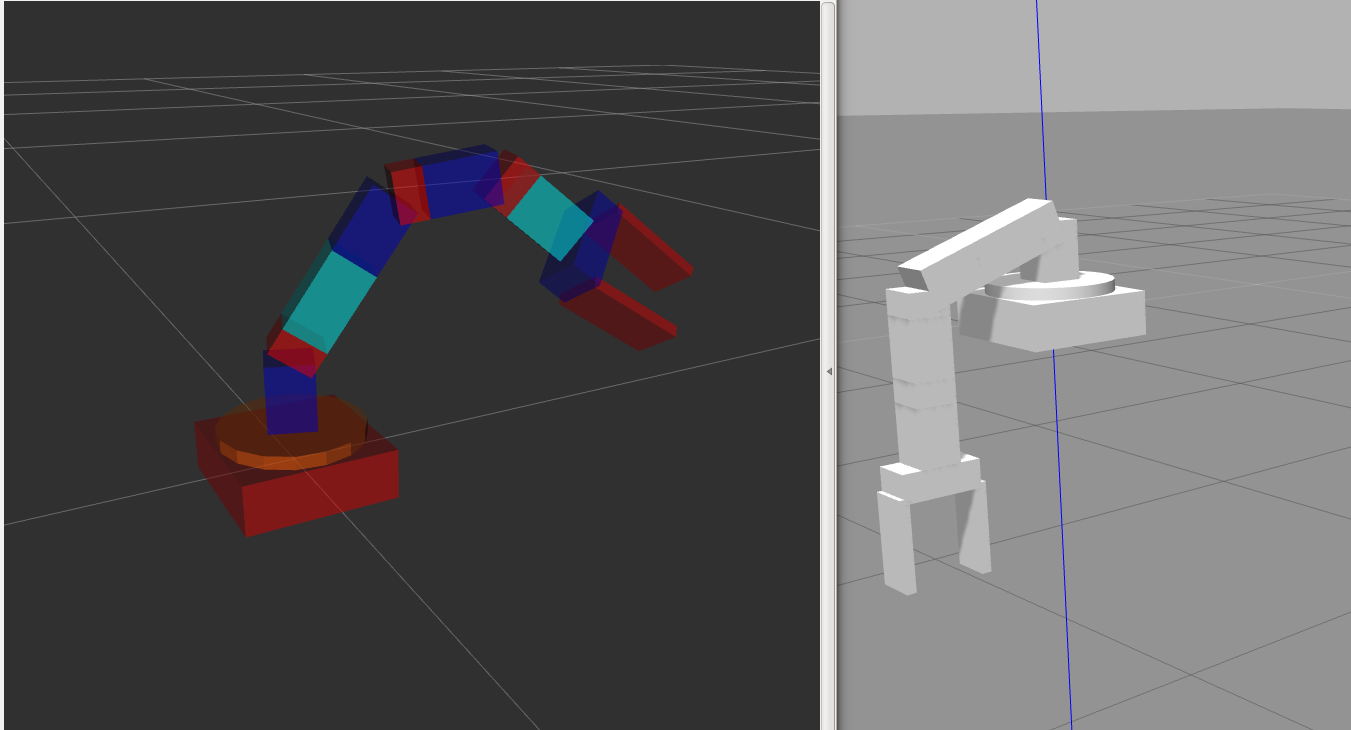
\includegraphics[width=.9\textwidth]{img/test.png}
  \caption{Manipulators visualized in Rviz and Gazebo, respectively}
  \label{fig:robot}
\end{figure}


\section*{Coding}
All the code can be found at this Github repository: \href{https://github.com/Aarskog/robotarm}{\underline{rotbotarm}}


\subsection*{Unified Robot Description Format (URDF)}
So far the model of the manipulator has been done using a Unified Robot Description Format (URDF) file. The syntax is very easy to understand. In \figref{fig:urdf_code_example} some code for the manipulator is given. This code decribes the mounting plates on the motors where the nect link can be mounted on. 
This particular code is a macro which means that it can be reused later in the code such that repeated code is avoided. The first part is the visuals for the plate. The mounting plate is illustrated as a box where length, width and height are specified. The next is collision which states the physical boundaries of the object. And the last is inertia where random inertia values are selected because Gazebo will not accept macroed values.


\begin{figure}[htbp]
  \centering
  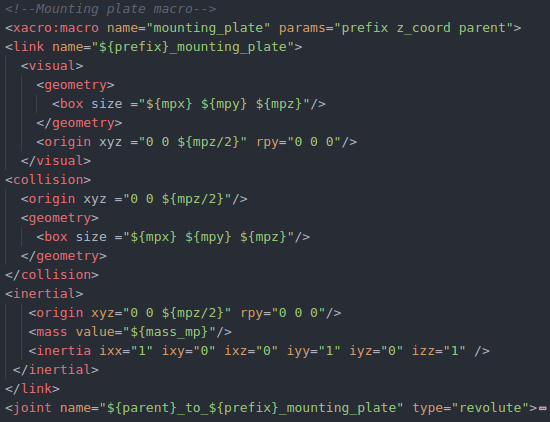
\includegraphics[width=.7\textwidth]{img/urdf_code_example.png}
  \caption{URDF-code example}
  \label{fig:urdf_code_example}
\end{figure}




\subsection*{YAML-file}
In the project, the joints.yaml file is the configuration file that states the torque controller for each joint. As per now a PID controller is used for each joint. This is based on a SISO system for each joint. The dynamic equations of the manipulator is in fact a complex nonlinear and multivariable system. 

\subsection*{Launch files}
The launch files are used for starting up Gazebo,Rviz and the different nodes. It is also used to place the robot model into the simulation environment. The controller nodes are launched form control.launch.





\subsection*{Python}
As per now a single python script is used for control of the manipulator. The task of the script is to listen to the Gazebo topic wich publishes the joint variables. 


\section*{Description of the Robot hand at hand}


\begin{figure}[htbp]
  \centering
  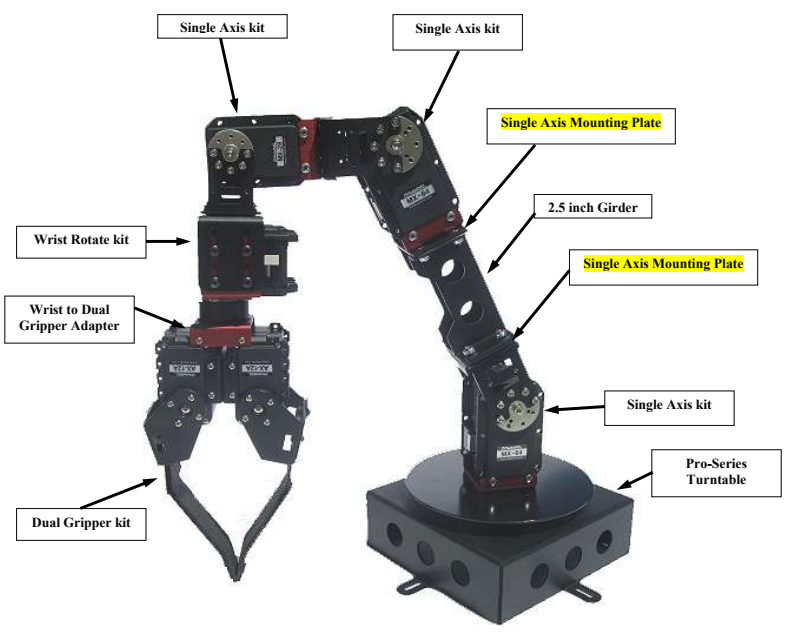
\includegraphics[width=.7\textwidth]{img/robotAH.png}
  \caption{Robot at hand}
  \label{fig:robotAH}
\end{figure}


\section*{Why use Gazebo to simulate the robot?}

\section*{Making a visual model to be used in Gazebo}
To make the visual model of the robot arm Unified Robot Description Format(URDF) is used. It is based on XML and is very easy to use although it has its limitations. It is not compatible with parallel linkages and it does not include friction among other things. It can not specify other objects which are not part of the robot. For this case the URDF works fine. The URDF includes mass and inertia as parameters which is possible to add a property of the joint. With this is mind the first to do is to find the mass of the different components that the robot at hand consists of. In \figref{fig:robotAH} for modelling and simulation the turntable base mass is not important to know since it is assumed that it is an unmoveable object that is stuck on the world frame. \\

\subsection*{Dviding the robot into parts}
For the robot to be properly modelled in the URDF file the robot has to split up into different parts. This must be done because the URDF file is constructed such that you build your robot in sequence from the bottom and up by adding part by part and states where it is and how it should behave in respect to its parent part. The parent of the first part is the world frame. In table \tabref{table:partlist} the different parts from the datasheet is listed. \tabref{table:partlist} is the initial list that was used as a base for constructing the robot. And in \figref{fig:utgangspunkt} the partnames are set their respective places on the robot. 

\begin{table}[h]
\centering
\caption{Partlist of the relevant parts taken from the datasheet and webpage of the robot}
\label{table:partlist}
    \begin{tabular}{ l r}
        \hline \\[-1em]
        Partname  & Amount \\
        \hline
        MX-28T Pro-Series Turntable & 1\\
        MX-64T Pro-Series Single Axis kits& 2\\
        Pro-Series Single Axis Mounting Plates & 3\\
        2.5 inch(6.35cm) Pro Series Girder & 1 \\
        MX-28T Pro-Series Single Axis kit & 1 \\
        MX-28T Pro-Series Wrist Rotate kit & 1\\
        Pro-Series Wrist to Dual Gripper Adapter & 1\\
        Dual gripper kit with two AX-12A Servos& 1\\
               \hline
    \end{tabular}
\end{table}



\begin{figure}[htbp]
  \centering
  \includesvg[width=.9\textwidth]{img/utgangpunktURDF.svg}
  \caption{Robot at hand}
  \label{fig:utgangspunkt}
\end{figure}



\subsection*{Finding and guesstimating weights}
All the other weights above the turntable must be known. Unfortunately the datasheet does not give specific information about all of the parts. More of items were found in the webstore, but not all. The rest had to be guesstimated. For example the mass of circular plate which the rest of the arm stands on is not given explicitly. In \tabref{table:partmass} the different masses of the parts are presented. 
\begin{table}[h]
\centering
\caption{Mass of parts}
\label{table:partmass}
    \begin{tabular}{l c r}
        \hline \\[-1em]
        Part  &  Weight(kg) & Estimated\\
        \hline
        MX-28T Pro-Series Turntable Plate& 0.05 & yes\\
        MX-64T Pro-Series Single Axis kits& 0.126 & no\\
        AX Short Bracket (SSB-Short) & 0.01 & yes\\
        2.5 inch(6.35cm) Pro Series Girder & 0.0227 & no\\
        MX-28T Pro-Series Single Axis kit & 0.072 & no \\
        MX-28T Pro-Series Wrist Rotate kit & 0.127 & no\\
        Pro-Series Wrist to Dual Gripper Adapter & 0.126 & yes\\
        Dual gripper kit with two AX-12A Servos& 0.01 & yes\\
        \hline
    \end{tabular}
\end{table}


\subsection*{Moments of inertia}
The next thing that was necessary to find, is the different moments of inertia of the robotarm. As seen from \figref{fig:robotAH} the different parts have different shapes and lengths so it can be a challenge to find the exact moments of inertia. A simplification is therefore needed. The simplifictaion that is used is to model them as boxes with uniform weight distribution. Although inertia is important to get a good model of the real robot, this simplifictation should not have a big impact of the error in the modelling. To calculate the moment of inertia the width,length and height of the part are needed. To simplify the naming of the different parts the following names seen in \figref{fig:naming} are used.\\


\begin{figure}[htbp]
  \centering
  \includesvg[width=.9\textwidth]{img/utgangpunktURDFWithNaming.svg}
  \caption{Naming}
  \label{fig:naming}
\end{figure}

\begin{table}[h]
\centering
\caption{Measurements of parts}
\label{table:measurements}
    \begin{tabular}{l c c c r}
        \hline \\[-1em]
        Part  &  x - Width(meter) & y - Length(meter) & z - Height(meter)\\
        \hline
        Base & 0.1143 & 0.1143 & 0.0381\\
        Turntable & 0.055(radius) & NA & 0.01\\
        Motor2345 & 0.0356 & 0.0355 & 0.0506 \\
        Bracket123 & 0.0356 & 0.0355 & 0.0206 \\
        Girder & 0.0356 & 0.0355 & 0.0635\\
        Adapter & 0.0356 & 0.0710 & 0.0253\\
        Left/right finger & 0.03568 & 0.0089 & 0.08\\
        \hline
    \end{tabular}
\end{table}


The complete documentation on the different parts is not complete this means that some of the lengths has to be guesstimated. In the simplified model (\figref{fig:naming}) there are only boxes except the turntable which is a small cylinder. For the boxes the following inertia matrix is used

\begin{align*}
    I = 
    \begin{bmatrix}
        I_{xx} & 0 & 0\\
        0 & I_{yy} & 0\\
        0 & 0 & I_{zz}
    \end{bmatrix}
\end{align*}
where
\begin{align*}
    I_{xx} &= \frac{1}{12}m(height^2+length^2)\\
    I_{yy} &= \frac{1}{12}m(height^2+width^2)\\
    I_{zz} &= \frac{1}{12}m(length^2+width^2)
\end{align*}
for the parts which are modelled as boxes and 
\begin{align*}
    I_{xx} &= \frac{1}{12}m(3r^2+height^2)\\
    I_{yy} &= \frac{1}{12}m(3r^2+height^2)\\
    I_{zz} &= \frac{1}{2}mr^2
\end{align*}
for the cylindrical turntable. 

\begin{table}[htbp]
\centering
\caption{Base is left out because it is fixed to the world frame and it is not neceassary to calculate this inertia}
\label{table:inertia}
    \begin{tabular}{l c c r}
        \hline \\[-1em]
        Part  &  $I_{xx}$ & $I_{yy}$ & $I_{zz}$\\
        \hline
        Turntable & $3.82\cdot10^{-5}$ &  $3.82\cdot10^{-5}$ &$2.27\cdot10^{-4}$\\
        Motor2345 & $4.01\cdot10^{-5}$  & $4.01\cdot10^{-5}$  & $2.65\cdot10^{-5}$ \\
        Bracket123 & $1.40\cdot10^{-6} $ & $1.40\cdot10^{-6} $ & $2.10\cdot10^{-6} $ \\
        Girder & $1.00\cdot10^{-5} $ & $1.00\cdot10^{-5} $ & $4.80\cdot10^{-6} $\\
        Adapter & $5.97\cdot10^{-5} $ & $2.00\cdot10^{-5} $ & $6.62\cdot10^{-5} $\\
        Left/right finger & $~0$ & $~0$ & $~0$\\
        \hline
    \end{tabular}
\end{table}

The moments of inertia are very small, and axis of rotation needs to be cheked. It is also unknown how the URDF reader uses the inertias and how much it is up to the user to do adjustments. 

\subsection*{Constructing the robot}
Now everything need to make the URDF file is found and the calculations needed to be done is done. 





%\section*{Path planning}


%\section*{Trajectory planning}
%The trajectory planner decides the joint velocites and accelerations while traversing the path. 
%\subsection*{Inverse kinematics}


